\documentclass[tikz,border=10pt]{standalone}
\usepackage{amsmath}
\usetikzlibrary{angles,quotes,calc}
\begin{document}
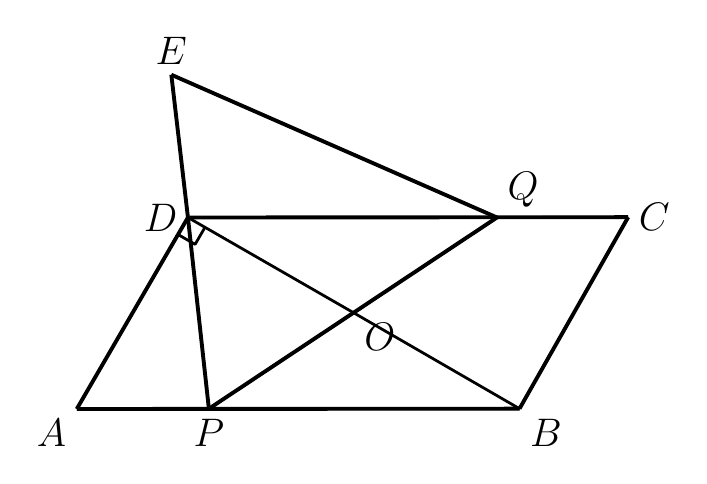
\begin{tikzpicture}[line join=round, line width=1.0pt, font=\fontsize{13.5}{16.2}\selectfont]
\coordinate (A) at (-3.526,-2.116);
\coordinate (B) at (2.097,-2.112);
\coordinate (C) at (3.477,0.320);
\coordinate (D) at (-2.114,0.316);
\coordinate (E) at (-2.325,2.129);
\coordinate (O) at (-0.008,-0.895);
\coordinate (P) at (-1.848,-2.113);
\coordinate (Q) at (1.811,0.316);



\draw[line width=1.4pt] (A) -- (B);
\draw[line width=1.4pt] (D) -- (C);
\draw[line width=1.4pt] (D) -- (A);
\draw[line width=1.4pt] (B) -- (C);
\draw[line width=1.4pt] (E) -- (Q);
\draw[line width=1.4pt] (P) -- (Q);


\draw (A) -- (P) -- (B);


\draw[line width=1.4pt] (E) -- (D) -- (P);

\draw (D) -- (O) -- (B);

\draw (P) -- (O) -- (Q);

\draw (D) -- (Q);
\draw (C) -- (Q);


\draw pic[draw, angle radius=0.250cm] {right angle=A--D--B};

\node[below left] at (A) {$A$};
\node[below] at (P) {$P$};
\node[below right] at (B) {$B$};
\node[left] at (D) {$D$};
\node[above right] at (Q) {$Q$};
\node[right] at (C) {$C$};
\node[above] at (E) {$E$};
\node[below right] at (O) {$O$};
\end{tikzpicture}
\end{document}